\chapter{Malware difundido en redes sociales}
\chapter{Phishing, estafas a través de la red}
\begin{tcolorbox}[
    title=Detalles de la Noticia, 
    colframe=black, % Borde azul oscuro
    colback=gray!5,         % Fondo gris claro
    sharp corners,          % Esquinas afiladas,
    breakable              % Permite que el cuadro se divida en varias páginas si es necesario
]

    % 1. Descripción y Título
    \textbf{Breve descripción de la amenaza:}
    \vspace{0.5em}
   
    \vspace{0.5em}

    \textbf{Fecha de la noticia:}
    \vspace{0.5em}
    02/07/2026
    \textbf{Título de la noticia:}
    \vspace{0.5em}
    \href{Los infostealers más presentes en Latinoamérica en 2025}{https://www.welivesecurity.com/es/malware/infostealers-presentes-latinoamerica-2025/}

    % 2. Enlaces y Medio
    \textbf{Enlace a la noticia:}
    \vspace{0.5em}
    \href{https://www.welivesecurity.com/es/malware/infostealers-presentes-latinoamerica-2025/}{https://www.welivesecurity.com/es/malware/infostealers-presentes-latinoamerica-2025/}

    \textbf{Medio:}
    \vspace{0.5em}
    Welivesecurity, blog de seguridad informática de la empresa de ciberseguridad ESET.

    \textbf{Enlace al medio:}
    \vspace{0.5em}
    \href{https://www.welivesecurity.com}{https://www.welivesecurity.com}

    \textbf{Nacionalidad del medio:}
    \vspace{0.5em}
    Bratislava, Eslovaquia.
    \textbf{Idioma de la noticia:}
    \vspace{0.5em}
    Español
    % 3. Imagen
    \textbf{Pequeña imagen de la noticia:}
    \newline
    \vspace{1em}
    \begin{minipage}{0.4\textwidth}
    \centering % Centra el contenido dentro del minipage
    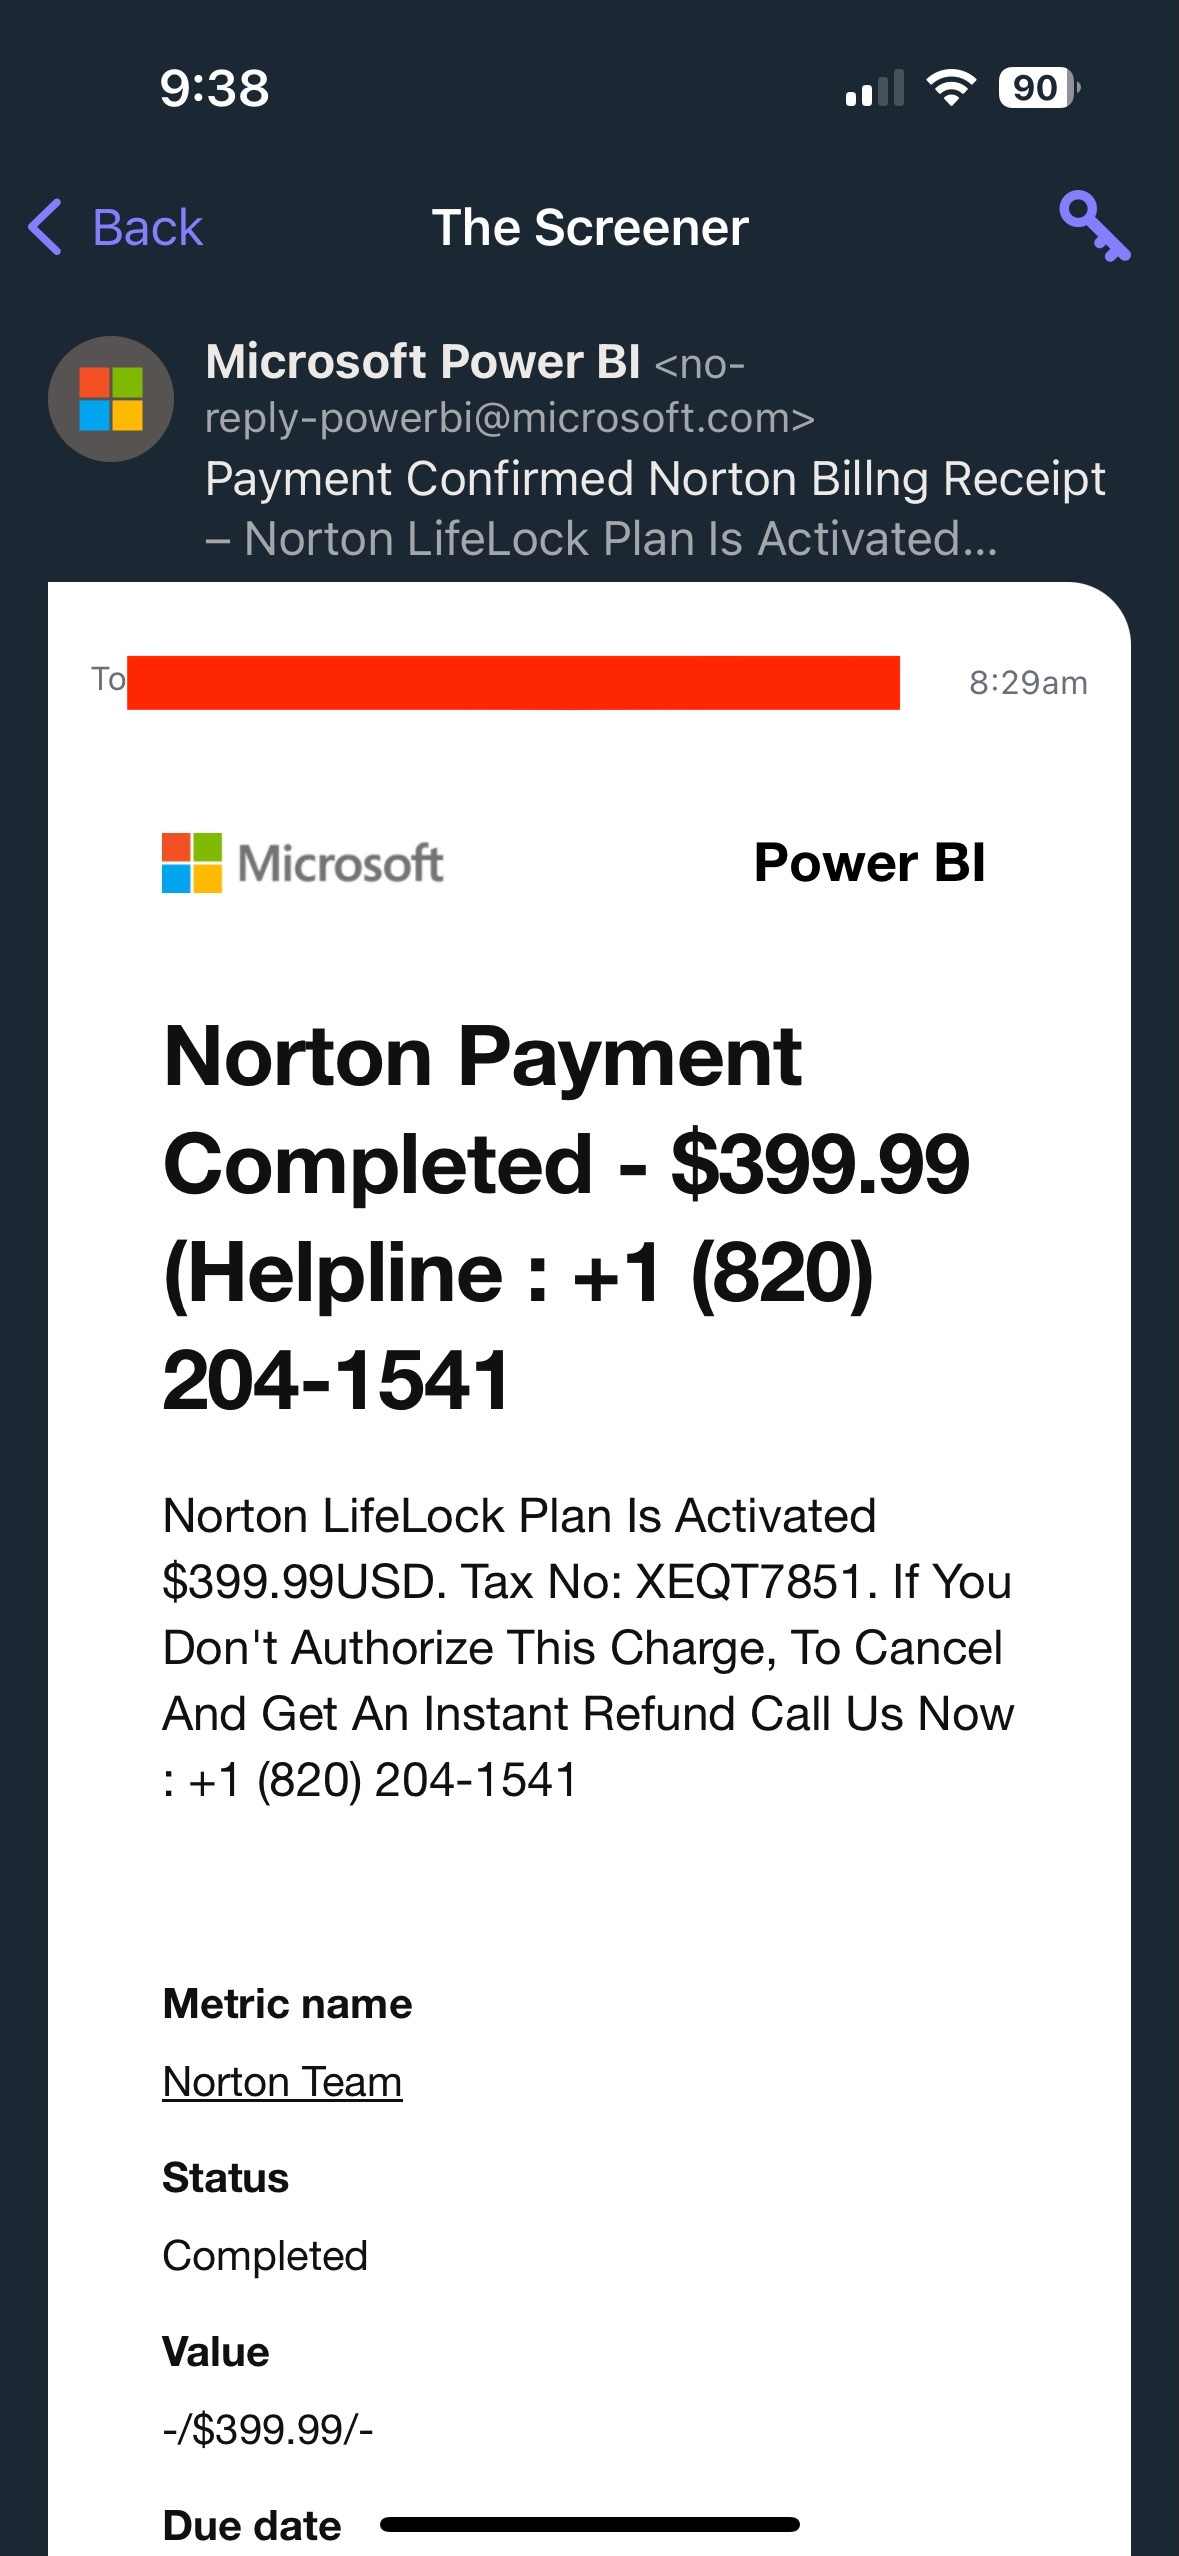
\includegraphics[width=\linewidth]{Imagenes/01-phishing.jpeg} 
    \end{minipage}
    \hfill
    \begin{minipage}{0.4\textwidth}
    \centering % Centra el contenido dentro del minipage
    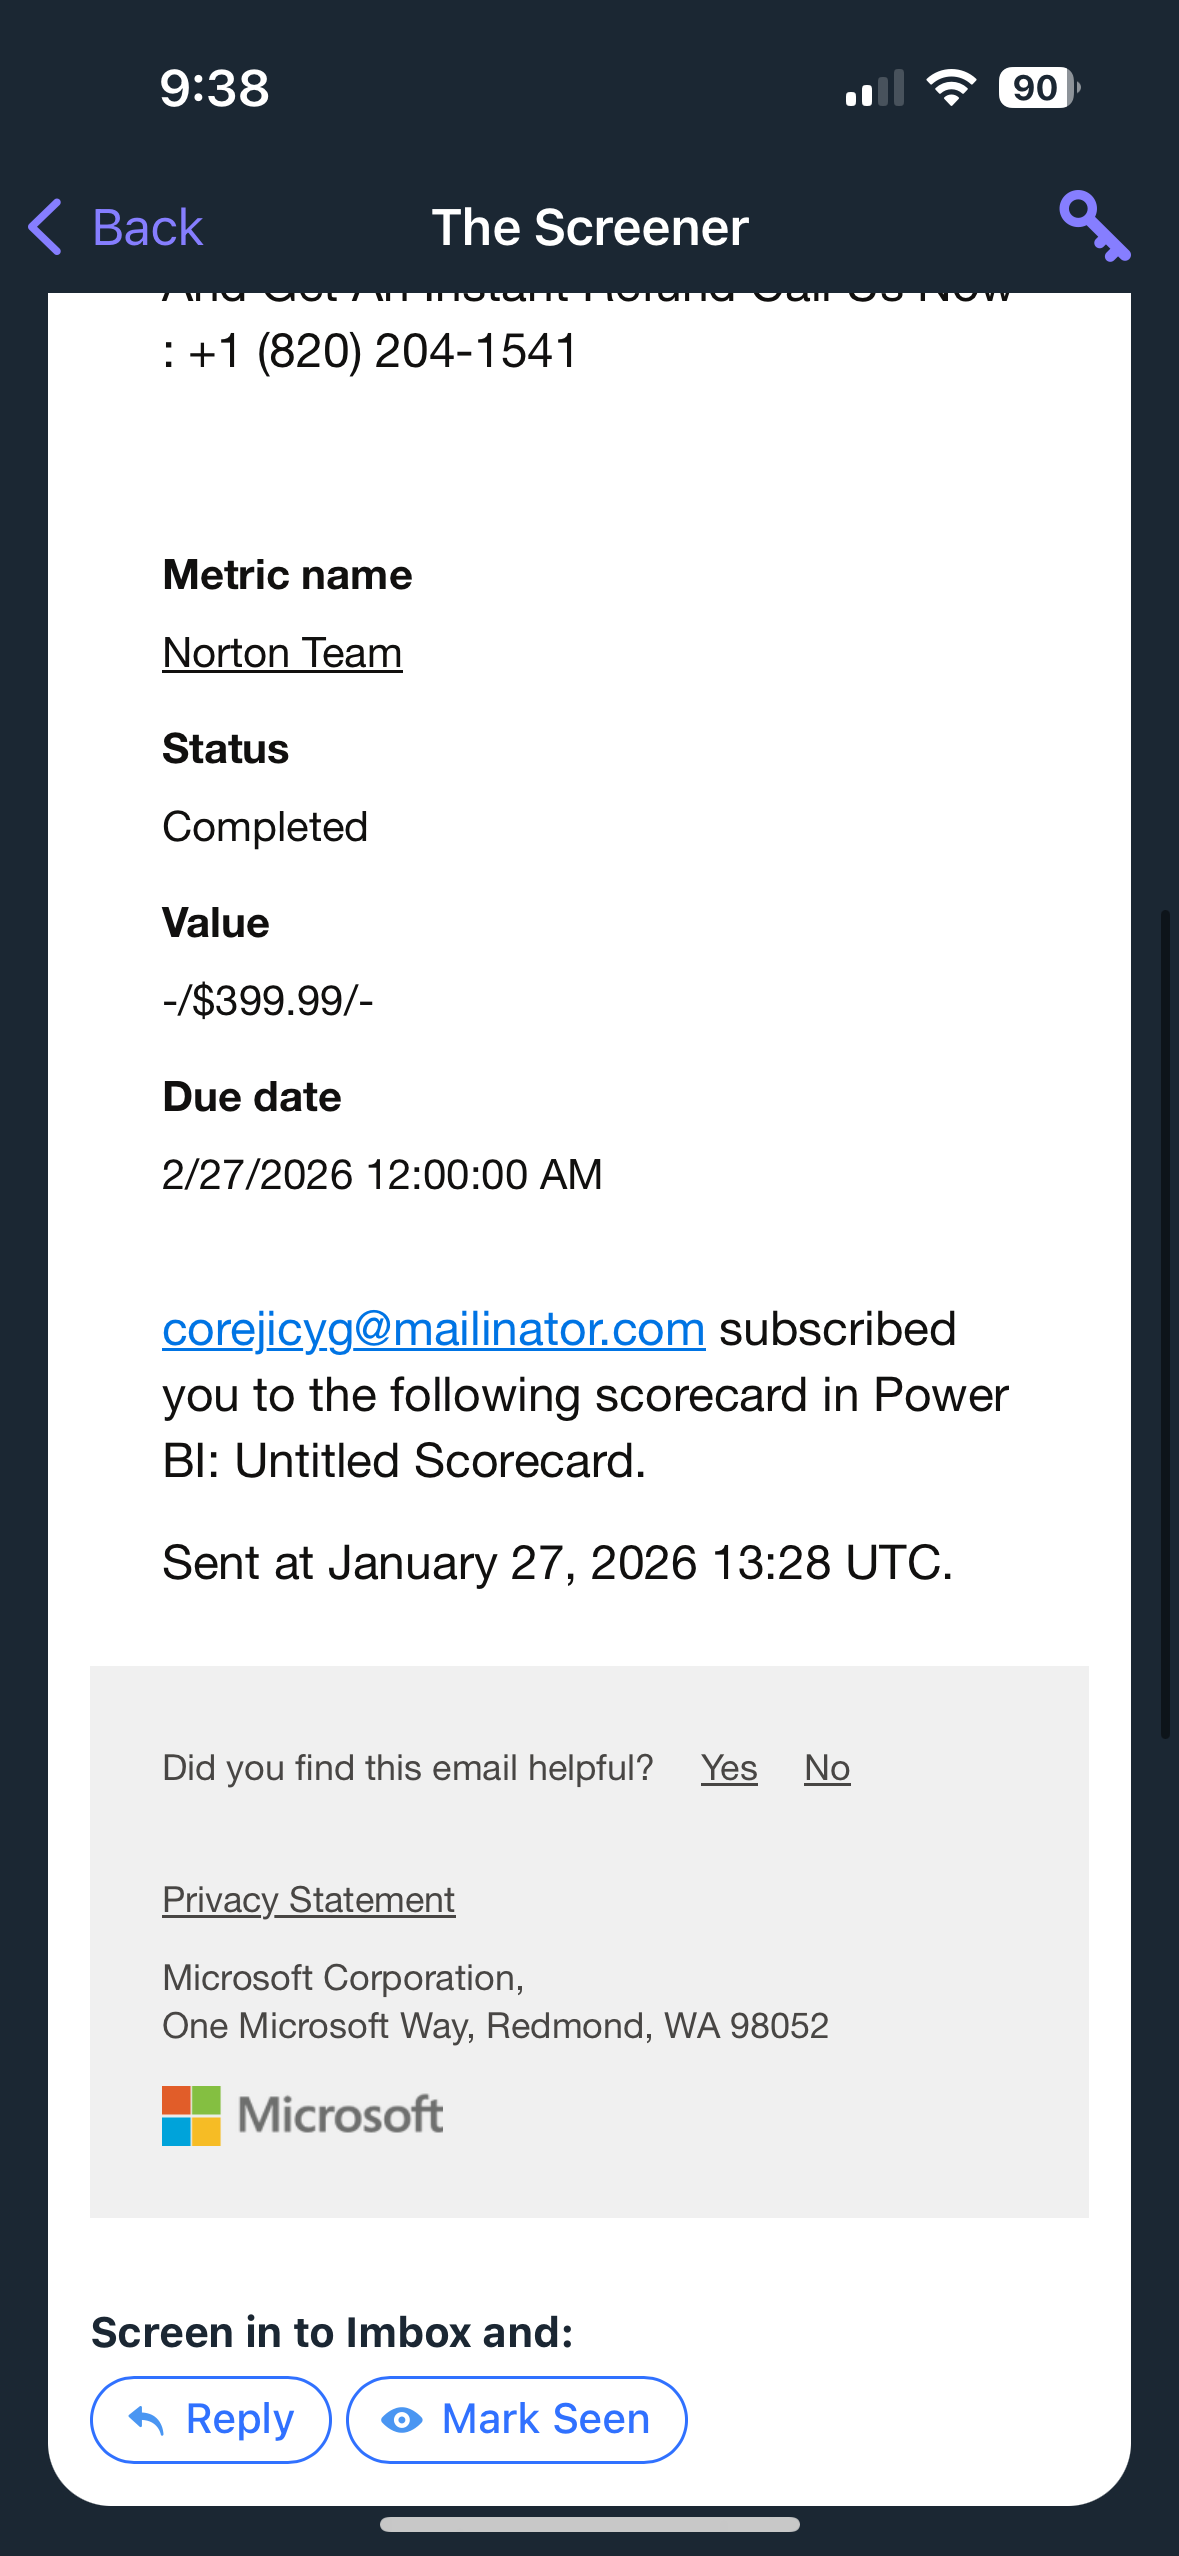
\includegraphics[width=\linewidth]{Imagenes/02-phishing.png}
    \end{minipage}

    % 4. Resumen y Análisis
    \textbf{Breve resumen de la noticia:}
    \vspace{0.5em}

    \textbf{Relación con la amenaza:}
    \vspace{0.5em}

    \textbf{\textquestiondown Existe CVE o CWE asociado a la noticia?}
    \vspace{0.5em}

    \textbf{Impacto ocasionado por la amenaza en esta noticia (más de 100 palabras):}
    \vspace{0.5em}

\end{tcolorbox}